%\title{LaTeX Portrait Poster Template}
%%%%%%%%%%%%%%%%%%%%%%%%%%%%%%%%%%%%%%%%%
% a0poster Portrait Poster
% LaTeX Template
% Version 1.0 (22/06/13)
%
% The a0poster class was created by:
% Gerlinde Kettl and Matthias Weiser (tex@kettl.de)
% 
% This template has been downloaded from:
% http://www.LaTeXTemplates.com
%
% License:
% CC BY-NC-SA 3.0 (http://creativecommons.org/licenses/by-nc-sa/3.0/)
%
%%%%%%%%%%%%%%%%%%%%%%%%%%%%%%%%%%%%%%%%%

%----------------------------------------------------------------------------------------
%   PACKAGES AND OTHER DOCUMENT CONFIGURATIONS
%----------------------------------------------------------------------------------------

\documentclass[a0,portrait]{a0poster}

\usepackage{multicol} % This is so we can have multiple columns of text side-by-side
\columnsep=100pt % This is the amount of white space between the columns in the poster
\columnseprule=3pt % This is the thickness of the black line between the columns in the poster

\usepackage[svgnames]{xcolor} % Specify colors by their 'svgnames', for a full list of all colors available see here: http://www.latextemplates.com/svgnames-colors

%\usepackage[colorgrid,texcoord]{eso-pic}

\usepackage{times} % Use the times font
%\usepackage{palatino} % Uncomment to use the Palatino font

\usepackage{graphicx} % Required for including images
\graphicspath{{figures/}} % Location of the graphics files
\usepackage{booktabs} % Top and bottom rules for table
\usepackage[font=small,labelfont=bf]{caption} % Required for specifying captions to tables and figures
\usepackage{amsfonts, amsmath, amsthm, amssymb} % For math fonts, symbols and environments
\usepackage{wrapfig} % Allows wrapping text around tables and figures

% apparently longtable package does not work in multi-column mode.
% use either xtab or supertabular instead
% Reference: https://tex.stackexchange.com/a/161455/2064
%\usepackage{supertabular,booktabs}
%\usepackage{longtable, booktabs}
\usepackage{xtab, booktabs}

\graphicspath{{figures/}}

%----------------------------------------------------------------------------------------
%	BIBLIOGRAPHY
%----------------------------------------------------------------------------------------

% Biblatex setup
% The default is the 'numerical' style.
\usepackage[backend=biber,url=false,eprint=true,doi=true,sorting=none,backref=true]{biblatex}
%\usepackage[backend=bibtex,url=false,eprint=true,doi=true,sorting=none,backref=true]{biblatex}
% We use the following bibliography databases:
\addbibresource{../../articles/timesarrow/timesarrow.bib}

% % % Custom Commands
\newcommand{\bite}{\begin{itemize}}
\newcommand{\eat}{\end{itemize}}
\newcommand{\beq}{\begin{equation}}
\newcommand{\eeq}{\end{equation}}
\newcommand{\rarrow}{\rightarrow}
%\newcommand{\bra}{\langle}
%\newcommand{\ket}{\rangle}
\newcommand{\beqa}{\begin{align}}
\newcommand{\eeqa}{\end{align}}
\newcommand{\barr}{\begin{array}}
\newcommand{\earr}{\end{array}}
\newcommand{\del}{\partial}
\newcommand{\de}{\mathrm{d}}
%\newcommand{\mu\nu}{{\mu\nu}}
\renewcommand{\th}{\mathrm{th}}
\newcommand{\com}[1]{\begin{itemize}\color{RED}{{#1}}\end{itemize}}
\newcommand{\C}{\mathbb{C}}
\newcommand{\R}{\mathbb{R}}
\newcommand{\btw}[1]{\color{PURPLE}{{#1}}\color{BLACK}}
\newcommand{\cut}[1]{\color{RED}{{#1}}\color{BLACK}}

%text
\newcommand{\ie}{\textit{i.e.}~}
\newcommand{\eg}{\textit{e.g.}~}
\newcommand{\wrt}{\textit{w.r.t.}~}
\newcommand{\etc}{\textit{etc.}~}


\newcommand{\M}{\mathcal{M}}
\newcommand{\N}{\mathcal{N}}
% \newcommand{\H}{\mathcal{H}}

\newcommand{\mb}[1]{\mathbf{#1}}
\newcommand{\mc}[1]{\mathcal{#1}}
\newcommand{\mbb}[1]{\mathbb{#1}}
\newcommand{\mf}[1]{\mathfrak{#1}}

\newcommand{\vect}[1]{\boldsymbol{#1}}
\newcommand{\expect}[1]{\langle #1\rangle}
\newcommand{\innerp}[2]{\langle #1 \vert #2 \rangle}
%\newcommand{\fullbra}[1]{\langle #1 \vert}
%\newcommand{\ket}[1]{\vert #1 \rangle}
\newcommand{\bra}[1]{\langle #1 \vert}
\newcommand{\ket}[1]{\vert #1 \rangle}
\newcommand{\supersc}[1]{$^{\textrm{#1}}$}
\newcommand{\subsc}[1]{$_{\textrm{#1}}$}
\newcommand{\sltwoc}{\mathfrak{sl}(2,\mathbb{C})}

\newcommand{\Tr}{\mathrm{Tr}}

% % %

\begin{document}

%----------------------------------------------------------------------------------------
%   POSTER HEADER 
%----------------------------------------------------------------------------------------

% The header is divided into two boxes:
% The first is 75% wide and houses the title, subtitle, names, university/organization and contact information
% The second is 25% wide and houses a logo for your university/organization or a photo of you
% The widths of these boxes can be easily edited to accommodate your content as you see fit

%\veryHuge {EVONET18 \hfill MPI-PKS, DRESDEN \hfill Jun 18 - 22, 2018} \\ [1cm]
\begin{minipage}{\linewidth}
\Large EVONET18 \hfill Max Plank Institut Für Physik Komplexer Systeme, Dresden \hfill Jun 18 - 22, 2018 \\ [1cm]
\end{minipage}

\begin{minipage}[b]{0.75\linewidth}
\veryHuge \color{NavyBlue} \textbf{Arrow of Time from \\ [0.5cm] Spontaneous Symmetry Breaking in LQG} \color{Black}\\[0.5cm] % Title
%\Huge\textit{An Exploration of Complexity}\\[2cm] % Subtitle
\huge \textbf{Deepak Vaid}\\[0.5cm] % Author(s)
\Large Department of Physics \\ National Institute of Technology Karnataka (NITK), India\\[0.4cm] % University/organization
\Large \texttt{dvaid79@gmail.com}\\
\end{minipage}
%
\hspace*{-5in}
\begin{minipage}[b]{0.125\linewidth}
\includegraphics[width=\linewidth]{evonet18_logo.png}
\end{minipage}
%\hspace*{-1in}
\begin{minipage}[b]{0.125\linewidth}
\includegraphics[width=\linewidth]{mpipks_logo.png}
\end{minipage}
\hspace*{0.5in}
\begin{minipage}[b]{0.125\linewidth}
\includegraphics[width=\linewidth]{nitk_logo_color_v1.png}
\end{minipage}

\vspace{1cm} % A bit of extra whitespace between the header and poster content

%----------------------------------------------------------------------------------------

\begin{multicols}{3} % This is how many columns your poster will be broken into, a portrait poster is generally split into 2 columns

%----------------------------------------------------------------------------------------
%   ABSTRACT
%----------------------------------------------------------------------------------------

\color{Navy} % Navy color for the abstract

%\large
%\normalsize

\begin{abstract}
%\large
The question of the origin time's arrow is a major outstanding problem in physics. Here we present a possible mechanism for generation of a cosmological arrow via spontaneous symmetry breaking in a theory of quantum gravity. In \cite{Chen2015Gauging}, Chen and Vishwanath have shown that a local notion of time-reversal symmetry can be encoded into a gauge field living on a tensor network. Using the fact that tensor networks can be used to describe the state space of Loop Quantum Gravity \cite{Qi2013Exact,Han2016Loop} we show that a spontaneous symmetry breaking mechanism operating on such tensor networks can lead to the spontaneous generation of an arrow of time corresponding to the generation of non-zero order parameter for the Chen-Vishwanath gauge field.

\end{abstract}

%----------------------------------------------------------------------------------------
%   INTRODUCTION
%----------------------------------------------------------------------------------------

%\large

%\color{SaddleBrown} % SaddleBrown color for the introduction
%
%\section*{Time-Reversal in Classical Mechanics}
%
%The effect of time-reversal on classical observables is given by:
%
%%\begin{figure}
%%	\centering
%\begin{center}
%%	\centering
%	\begin{xtabular}{l|l}
%	\toprule
%	Physical Observables & Under time reversal\\
%	\midrule
%	Position &  $ \vect{x} \rightarrow \vect{x} $ \\
%	Time & $  t \rightarrow -t$\\
%	Linear Momentum & $ \vect{p} \rightarrow -\vect{p} = d\vect{x}/d(-t) = - d\vect{x}/dt$\\
%	Angular Momentum & $  \vect{l} = \vect{x} \times \vect{p} \rightarrow -\vect{l} $ \\
%	Energy/Hamiltonian & $  H(\vect{x},\vect{p}) \rightarrow H(\vect{x}, -\vect{p}) $ \\
%	Electric Field & $  E^i \rightarrow -E^i$\\
%	Magnetic Field & $  B^i \rightarrow - B^i $\\
%	\bottomrule
%	%\captionof{table}{\color{Green} Table caption}
%	\end{xtabular}
%\end{center}
%\end{figure}

%\color{DarkSlateGray} % DarkSlateGray color for the rest of the content

%\color{Navy}

%\color{Indigo}

%\color{DarkGreen}

\color{DarkRed}

\section*{Time Reversal in Quantum Mechanics}

\begin{center}
%	\centering
	\begin{xtabular}{l|c}
	\toprule
	Operators: & $ \vect{\hat{x}} \rightarrow \vect{\hat{x}}; \quad \vect{\hat{p}} \rightarrow -\vect{\hat{p}} $ \\
	Commutators: & 	$ \left[ \hat{x}_i, \hat{p}_j \right] = i \hbar \delta_{ij} \rightarrow \left[\hat{x}'_i, \hat{p}'_j \right] = - i \hbar \delta_{ij} $ \\
	Equation of motion & $ i \hbar \frac{\partial \psi}{\partial t} =  \hat{H} \psi \rightarrow i \hbar \frac{\partial \psi}{\partial t'} =  - \hat{H} \psi $ \\
	\bottomrule
	\end{xtabular}
\end{center}

where $ t' = -t $. Define Wigner quantum time reversal operator:
\begin{equation}\label{eqn:wigner-time-reversal}
	\mc{T} ( c_1 \psi_1 + c_2 \psi_2 ) = c_1^* \mc{T} \psi_1 + c_2^* \mc{T} \psi_2
\end{equation}
Such an operator is called \emph{anti-linear} or \emph{anti-unitary}. Acting with this operator on both sides of the Schrodinger equation we obtain:
\begin{equation}\label{eqn:trs-schrodinger-2}
	\mc{T} \left( i \hbar \frac{\partial \psi}{\partial t} \right) = i \hbar \frac{\partial (\mc{T} \psi)}{\partial t'} = H (\mc{T} \psi)
\end{equation}
Under $ \mc{T} $, the quantum commutators no longer change sign:
\begin{equation}\label{eqn:quantum-poisson-2}
	\mc{T} \left(\left[ \hat{x}_i, \hat{p}_j \right]\right) \mc{T}^{-1} = \mc{T} i \mc{T}^{-1} \hbar \delta_{ij} \rightarrow \left[\hat{x}'_i, \hat{p}'_j \right]= i \hbar \delta_{ij}
\end{equation}

%----------------------------------------------------------------------------------------
%   OBJECTIVES
%----------------------------------------------------------------------------------------

\vspace*{-1cm}

%\color{SaddleBrown}

%\color{DarkRed}

\color{DarkGreen}

%\color{DeepPink}

\section*{Time Reversal of Many Body State}

\begin{equation}\label{eqn:many-body-state}
	\ket{\psi} = \sum_{i_1, i_2, \ldots, i_N} C_{i_1, i_2, \ldots, i_N} \ket{i_1, i_2, \ldots, i_N}
\end{equation}
Co-efficients $  C_{i_1, i_2, \ldots, i_N} $ are defined over the entire Hilbert space and cannot be decomposed into local contributions in any simple manner. Global action of time-reversal is well defined
\begin{equation}\label{eqn:trs-many-body-state}
	\mc{T} \ket{\psi} = \sum_{i_1, i_2, \ldots, i_N} C^*_{i_1, i_2, \ldots, i_N} U_1 \otimes \ldots \otimes U_N \ket{i_1, i_2, \ldots, i_N}
\end{equation}
but local action is not clear, because $ C_{i_1, i_2, \ldots, i_N} $ cannot be simply split into sum of local pieces. To do so, we need matrix product states.

%----------------------------------------------------------------------------------------
%   MATERIALS AND METHODS
%----------------------------------------------------------------------------------------

%\color{DarkSlateGray}

\color{Navy}

\section*{Matrix Product State}

Following Bridgeman and Chubbs \cite{Bridgeman2016Hand-waving}:
\begin{equation}\label{eqn:mps-ansatz}
	\ket{\psi} = \sum_{i_1, i_2, \ldots, i_N} \Tr\left[ A^{(1)}_{i_1} A^{(2)}_{i_2} \ldots A^{(N)}_{i_N} \right] \ket{i_1, i_2, \ldots, i_N}
\end{equation}

\vspace*{2cm}

\begin{minipage}[m]{0.4\columnwidth}
	\centering
	\includegraphics[width=0.5\linewidth]{mps-vertex}
%	\captionof{figure}{Single vertex of a matrix product state. Internal indices are denoted by $ \alpha, \beta $. Physical indices by $ i,j,\ldots $}
	\label{fig:mps-vertex}
\end{minipage}
\begin{minipage}[m]{0.4\columnwidth}
	$ A^k_{i_k;\alpha\beta} $: Single vertex of a matrix product state. Internal indices are denoted by $ \alpha, \beta $. Physical indices by $ i,j,\ldots $
\end{minipage}

\vspace*{2cm}

\begin{minipage}[m]{0.45\linewidth}
	\centering
	\includegraphics[width=0.6\linewidth]{mps-vertex-product}
	\captionof*{figure}{A connection between two adjacent vertices corresponds to multiplying the associated matrices.}
	\label{fig:mps-vertex-product}
\end{minipage}
\begin{minipage}[m]{0.45\linewidth}
	\centering
	\includegraphics[width=0.6\linewidth]{mps-vertex-product-trace}
	\captionof*{figure}{To take the trace we complete the loop by connecting the first and last vertices}
	\label{fig:mps-vertex-product-trace}
\end{minipage}

%\begin{minipage}[t]{\linewidth}
%\begin{align}
\begin{minipage}[m]{0.3\columnwidth}
	$$ \ket{\psi} = \sum_{i_1, i_2, \ldots, i_5} \Tr\left[ A^{(1)}_{i_1} A^{(2)}_{i_2} \ldots A^{(N)}_{i_5} \right] \ket{i_1, i_2, \ldots, i_5} = $$
\end{minipage}
\begin{minipage}[m]{0.4\columnwidth}
	\hspace*{8cm}\includegraphics[width=1.0\linewidth]{mps-state}
\end{minipage}
%	 & = \vspace*{2cm}\includegraphics[width=0.5\linewidth]{mps-state} \nonumber
%\end{align}
%	\includegraphics[width=0.7\linewidth]{mps-state}
%\end{minipage}

%\vfill
%\vspace*{2cm}

\color{DarkRed}

\section*{Tensor Network State on Arbitrary Graphs}

\begin{center}
	\begin{tabular}{|c|c|p{14cm}|}
		\toprule
		Vertex Tensors & $ T^v_{i_v; \alpha_1 \ldots \alpha_{v_k}} $ & $ v: $ vertex \newline $i_v$: vertex state/physical index \newline $\alpha_1 .. \alpha_k$: internal (``bond'') indices \\
		\midrule
		Edge Tensors & $ g^e_{i_e; \alpha\beta} $ &  $ e $: edge label \newline $i_e:$ edge state/physical index \newline $\alpha, \beta $: bonding indices \\
		\bottomrule
	\end{tabular}
\end{center}

%\begin{minipage}{0.4\columnwidth}
%\mbox{
%\begin{equation*}
%\end{equation*}
%}
%\end{minipage}

%\vspace*{0.5cm}
\resizebox{\columnwidth}{!}{ \framebox{ $
\ket{\Psi} = \underset{\{i_1,\ldots,i_{n_v}\}, \{ j_1,\ldots,j_{n_e} \}}{\sum} \Tr\left[ \underset{v \in \Gamma}\prod T^v_{i_v} \underset{e \in \Gamma}\prod g^e_{j_e} \right] \ket{i_1,\ldots,i_{n_v}; j_1, \ldots, j_{n_e} } $
}}

%\vspace*{-57pt}

\columnbreak

%\color{Navy}

\color{DarkGreen}

\section*{Dangling Indices: Bulk vs Boundary d.o.f.}

\normalsize

States with \emph{\textbf{dangling indices}}, \ie physical degrees of freedom which are not traced over, represent physical states of quantum geometry. Consider the MPS for a two-site system as before:

%\vspace*{1cm}

\begin{minipage}[m]{0.45\linewidth}
	\centering
	\includegraphics[width=0.7\linewidth]{mps-vertex-product}
%	\captionof*{figure}{}
%	\label{fig:mps-vertex-product}
\end{minipage}
\begin{minipage}[m]{0.45\linewidth}
%	\centering
	$$ \ket{\Psi_{\alpha\beta}}= \sum_{\{i_1, i_2\}} A^1_{i_1;\alpha\gamma} A^2_{i_2;\gamma\beta} \ket{i_1, i_2} $$
\end{minipage}
Now the state is a two-index object. Likewise if the graph has $ n $ dangling edges, then the resulting state will also have $ n $ indices of size equal to the bond dimension. Consider a graph $ \Gamma $, which has a subset of $ n $ vertices which are connected to only a single edge, each. These vertices and their accompanying edges $ \{ v_1,\ldots,v_n; e_1, \ldots, e_n \} $ form a subset $ \partial \Gamma \subset \Gamma $. Let $ \bar{\Gamma} = \Gamma/\partial \Gamma$, be the ``bulk'' of the graph which does not have any dangling edges. Resulting state is $ n $ index object.

\vspace*{1cm}
\begin{center}
\resizebox{0.6\columnwidth}{!}{ \framebox{ $
\ket{\Psi_{\alpha_1,\ldots,\alpha_n}} = \ket{\Psi_\text{bulk}}\ket{\alpha_1,\ldots,\alpha_n} $
}}
\end{center}

where:
\begin{center}
\resizebox{0.6\columnwidth}{!}{ \framebox{ $ \ket{\Psi_\text{bulk}} = \underset{\{i_v,j_e\} \in \bar{\Gamma}}{\sum} \left[ \underset{v \in \bar\Gamma}\prod T^v_{i_v} \underset{e \in \bar\Gamma}\prod g^e_{j_e} \right] \ket{ \{ i_v \}, \{ j_e \} } $
}}
\end{center}

%\columnbreak

\color{Black}

%\color{DarkGreen}

%\large

\section*{Gauge Transformations}

\begin{minipage}[m]{0.35\linewidth}
	\centering
	\includegraphics[width=\linewidth]{mps-gauge-action-v2}
	\captionof*{figure}{Global gauge rotation of two-site MPS state}
\end{minipage}
=
\begin{minipage}[m]{0.3\linewidth}
	\includegraphics[width=\linewidth]{mps-gauge-action-v3}
	\captionof*{figure}{All the rotations in the interior cancel out and we are left with only two occurrences at the either end of the chain.}
\end{minipage}
=
\begin{minipage}[m]{0.3\columnwidth}
	\includegraphics[width=0.6\linewidth]{mps-gauge-action-v4}
	\captionof*{figure}{On taking the trace, the remaining two matrices cancel, leaving us the original state.}
\end{minipage}

%\vfill
\vspace*{2cm}

\begin{minipage}[m]{0.45\columnwidth}
	\centering
	\includegraphics[width=0.6\linewidth]{mps-gauge-action}
	\captionof*{figure}{Action of gauge rotation on single site of MPS: $ A^1~\rightarrow~M (A^1) M^{-1} $}
\end{minipage}
\begin{minipage}[m]{0.45\columnwidth}
	\centering
	\includegraphics[width=1\linewidth]{local-symmetry-flux}
	\captionof*{figure}{Insertion of a single symmetry flux: $ A^2 \rightarrow M (A^2) $}
\end{minipage}

%\color{DarkGreen}

\color{DarkRed}

\section*{Gauging Time Reversal Symmetry}

\normalsize

Action of time-reversal on a \emph{single} system: $ \mc{T} = UK $, where $ K $ is complex conjugation, and $ U $ is some unitary.

For a single spin $ U = i\sigma_y $. State $ \ket{\psi} = \alpha \ket{0} + \beta \ket{1} \rightarrow i\sigma_y \ket{\psi}^* = \alpha^* \ket{1} - \beta^*\ket{0} $

Local TRS action on $ k^\text{th} $ site of MPS:

\vspace*{1cm}

\resizebox{\columnwidth}{!}{ \framebox{
$ \mc{T}_k \ket{\Psi}_{MPS} = \sum_{i_1, i_2, \ldots, i_N} \Tr\left[ A^{1}_{i_1},\ldots,\tilde{A}^k,\ldots, A^{N}_{i_N} \right] \ket{i_1, \ldots, (i\sigma_y) i_k, \ldots, i_N} $
}
}

\vspace*{1cm}

where $ \tilde{A}^k = (iY)(A^{k})(-iY) $

%\vspace*{1cm}

%------------------------------------------------

%\color{DarkSlateGray}

\color{Navy}

%\color{DarkGreen}

%\color{SaddleBrown}
\begin{minipage}[t]{0.45\linewidth}
	\includegraphics[width=0.9\columnwidth]{symmetry-flux-line-2d}
	\captionof*{figure}{Applying constant gauge transformation to given region, leaves symmetry flux insertions along boundary of region.}
\end{minipage}
\begin{minipage}[t]{0.45\linewidth}
	\includegraphics[width=0.9\columnwidth]{symmetry-flux-twist-2d}
	\captionof*{figure}{Insertion of a symmetry flux twist only along one line}
\end{minipage}

\section*{Spin Networks}

\begin{minipage}[m]{0.45\linewidth}
	\centering
	\includegraphics[width=0.6\linewidth]{spin-net-vertex}
%	\captionof*{figure}{}
\end{minipage}
\begin{minipage}[m]{0.45\linewidth}
	\small
	Illustration of a four-valent spin-network vertex.
	
	Each edge is labelled with a representation $ j_k $ of $ SU(2) $.
	
	Face area: $ 8\pi\gamma l_p^2 \sqrt{j_k (j_k + 1)} $.
	
	Vertex label: $ I_v \in \text{Inv}\left[\bigotimes_{i=1}^{4} \mc{H}^{j_k} \right] \equiv \mc{H}_{\text{Inv}}$
\end{minipage}

\vspace*{1cm}

\section*{Spin Network State on Arbitrary Graphs}

\begin{center}
	\begin{tabular}{|c|c|p{14cm}|}
		\toprule
		Vertex Tensors & $ I^v_{i_v; \alpha_1 \ldots \alpha_{v_k}} $ & $ v: $ vertex \newline $i_v$: vertex state/physical index \newline $\alpha_i \in \{ 1,..,d_i \} $; $ d_i = 2 j_i + 1 $: contracts with the state on the $ i^\text{th} $ edge joined to the vertex. \\
		\midrule
		Edge Tensors & $ D^e_{j_e; \alpha\beta} $ &  $ e $: edge \newline $j_e:$ $ SU(2) $ label of edge \newline $\alpha, \beta \in \{1,\ldots,(2 j_e + 1) \} $: bonding indices \\
		\bottomrule
	\end{tabular}
\end{center}

\resizebox{\columnwidth}{!}{ \framebox{ $
\ket{\Psi} = \underset{\{i_v\}, \{ j_e \}}{\sum} \Tr\left[ \underset{v \in \Gamma}\prod I^v_{i_v} \underset{e \in \Gamma}\prod D^e_{j_e} \right] \ket{i_1,\ldots,i_{n_v}; j_1, \ldots, j_{n_e} } $
}}

\columnbreak

\section*{Geometry from Spin Networks}

\begin{minipage}[t]{0.45\linewidth}
	\centering
%	\vspace{1cm}
	\includegraphics[width=0.5\linewidth]{area_puncture}
	\captionof*{figure}{Quantum of area from single puncture}
%	\vspace{1cm}
\end{minipage}
\begin{minipage}[t]{0.45\linewidth}
	\centering
%	\vspace{1cm}
	\includegraphics[width=0.6\linewidth]{area_punctures}
	\captionof*{figure}{Many punctures generate macroscopic areas}
%	\vspace{1cm}
\end{minipage}

\section*{CZX State - SPT with $ Z_2 $ Order in 2D}

\begin{minipage}[m]{0.3\linewidth}
	\includegraphics[width=0.9\linewidth]{czx_3by3_lattice}
\end{minipage}
\begin{minipage}[m]{0.65\linewidth}
	CZX model \cite{Chen2011Symmetry,Chen2010Local} is example of 2D SPT phase with $ Z_2 $ symmetry. \newline
	4 spins at each site; 4 neighboring spins form a plaquette. \newline
	State is invariant under \emph{\textbf{local}} action of of $ U_{CZX} $ at each vertex
\end{minipage}

\vspace*{1cm}

\begin{minipage}[m]{0.3\linewidth}
	\includegraphics[width=0.6\linewidth]{czx_vertex_labelled}
\end{minipage}
\begin{minipage}[m]{0.65\linewidth}
	$ U_{CZX} = U_X U_{CZ} $ \newline
	$ U_X = X_1 \otimes X_2 \otimes X_3 \otimes X_4 $ \newline
	$ U_{CZ} = (CZ)_{12} (CZ)_{23} (CZ)_{34} (CZ)_{41} $ \newline
	$ CZ = \ket{00}\bra{00} + \ket{01}\bra{01} + \ket{10}\bra{10} - \ket{11}\bra{11} $
\end{minipage}

\vspace*{1cm}

\begin{minipage}[m]{0.3\linewidth}
	\includegraphics[width=0.4\linewidth]{czx_plaquette}
\end{minipage}
\begin{minipage}[m]{0.65\linewidth}
	Each plaquette is in an entangled state: $ \ket{0000} + \ket{1111}$
\end{minipage}

\vspace*{1cm}

\subsection*{Prescription for $ Z_2 $ SPT State for Quantum Geometry }

\begin{enumerate}
	\item Join spin-network 4-valent vertices to make a square lattice.
	\item Enforce $ U_{CZX} $ symmetry at each site to generate SPT $ Z_2 $ state.
	\item Check that resulting state satisfies LQG constraints.
\end{enumerate}


%----------------------------------------------------------------------------------------
%   CONCLUSIONS
%----------------------------------------------------------------------------------------

%\color{SaddleBrown} % SaddleBrown color for the conclusions to make them stand out

%\color{DarkBlue}

%\color{SaddleBrown}

\color{DarkGreen}

\section*{Discussion}

\begin{enumerate}
	\item Time-reversal symmetry breaking happens due to formation of $ Z_2 $ domains in spin-networks.
	\item At ``high temperatures'', state will be disordered with no emergent macroscopic geometry.
	\item As temperature is lowered, macroscopic volume and area states emerge
	\item Accompanied by the formation of $ Z_2 $ domains which violate time-reversal symmetry.
	\item To identify semiclassical field which leads to $ Z_2 $ symmetry in GR.
\end{enumerate}

%\color{DarkSlateGray} % Set the color back to DarkSlateGray for the rest of the content

 %----------------------------------------------------------------------------------------
%   REFERENCES
%----------------------------------------------------------------------------------------

%\nocite{*} % Print all references regardless of whether they were cited in the poster or not
%\bibliographystyle{plain} % Plain referencing style
%\bibliography{../../articles/bib_library} % Use the example bibliography file sample.bib


%----------------------------------------------------------------------------------------
%   ACKNOWLEDGEMENTS
%----------------------------------------------------------------------------------------

\color{DarkRed}

\section*{Acknowledgements}

I thank IUCAA (Inter-University Centre for Astronomy and Astrophysics) located in Pune, India, for their support and hospitality under the ``Visiting Associate'' program, where this work was undertaken. I thank NITK, Surathkal for support under CPDA travel grant.

%----------------------------------------------------------------------------------------

\color{Navy}

\printbibliography[title={References}]

\end{multicols}
\end{document}